\begin{figure*}[t]
    \centering
    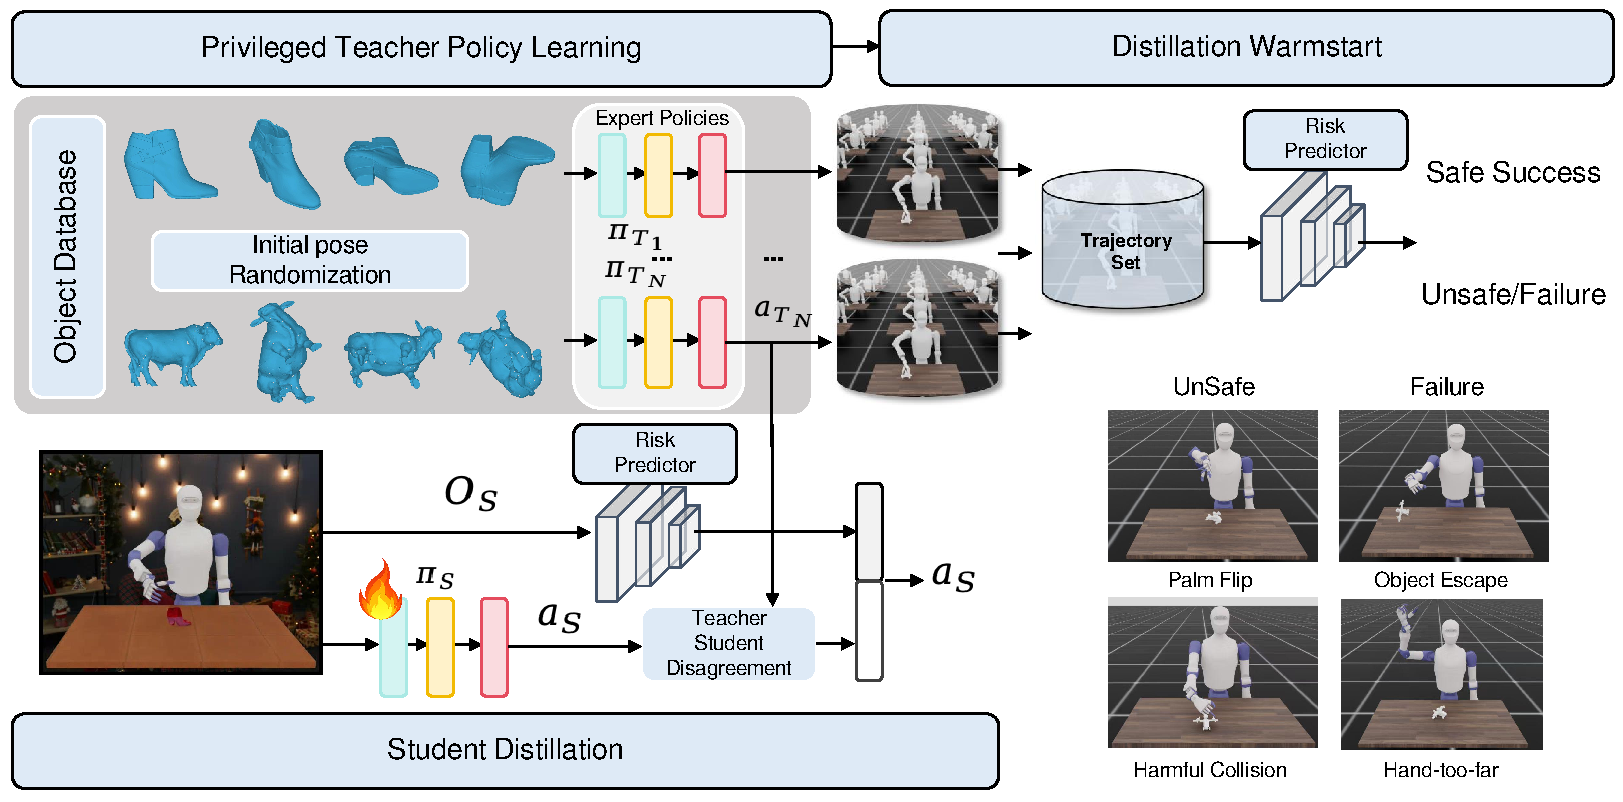
\includegraphics[width=0.8\linewidth]{figures/fig02_network_structure.pdf}
    \par\redtodo{TODO: Update Figure 2.}
    \caption{Overview of the proposed teacher--student learning pipeline. A
    privileged reinforcement learning teacher is trained in simulation and
    subsequently distilled into an RGB-based visuomotor policy for real-world
    deployment. \revision{A vision-language model periodically calibrates the
    intervention thresholds.}}
    \label{fig:pipeline}
\end{figure*}

\subsection{Problem Formulation}
We consider online interactive imitation learning with teacher intervention in a
partially observable Markov decision process (POMDP)
$\mathcal{M}=(\mathcal{S},\mathcal{A},\mathcal{O},P,\Omega,r,\gamma)$, with
privileged teacher state $s_t\in\mathcal{S}$, deployable student observation
$o_t\in\mathcal{O}$ (RGB), action $a_t\in\mathcal{A}$, observation model
$o_t\sim\Omega(\cdot\mid s_t)$, and dynamics
$s_{t+1}\sim P(\cdot\mid s_t,a_t)$. During training, we assume access to a set
of privileged teacher policies $\{\pi_{T_i}\}_{i=1}^{K}$, whereas at deployment
the student policy $\pi_S$ must act solely from $o_t$. Our goal is to distill
the collective teacher behavior into an RGB-based student that achieves high
task success while minimizing unsafe exploration during training.

The induced rollout distribution $p_{\pi_{\mathcal{G}}}$ is defined by the gated rollout policy
$\pi_{\mathcal{G}}$, which switches between the teacher and student policies
according to the intervention gate. Its learning objective and VLM-calibrated
gate are
\begingroup
\small
\begin{equation}
\begin{aligned}
\min_{\substack{\pi_S\in\Pi_S\\ \mathcal{G}\in\mathfrak{G}}}
\;
&
\Bigg[
\underbrace{
-\mathbb{E}_{\tau\sim p_{\pi_{\mathcal{G}}}}\!\left[\mathbb{I}_{\mathrm{succ}}(\tau)\right]
}_{\text{maximize success}}
\;+\;
\lambda\,
\underbrace{
\mathbb{E}_{\tau\sim p_{\pi_{\mathcal{G}}}}\!\left[
\sum_{t=0}^{T-1}\mathbb{I}_{\mathrm{unsafe}}(s_t,a_t)
\right]}_{\text{minimize unsafe}}
\Bigg]
\\
\text{s.t.}\quad
&
a_t=g_t a_t^T+(1-g_t)a_t^S,\\
&
g_t=\mathcal{G}(s_t,o_t)\in\{0,1\},\\
&
s_{t+1}\sim P(\cdot\mid s_t,a_t),\qquad
o_t\sim\Omega(\cdot\mid s_t).
\end{aligned}
\label{eq:vc_objective}
\end{equation}
\endgroup
where $g_t=1$ indicates teacher takeover and $g_t=0$ denotes student control.
\revision{The intervention gate $\mathcal{G}$ and its VLM-calibrated thresholds
are described in Secs.~E--F.}

We formalize task success via a trajectory-level predicate
$\mathbb{I}_{\mathrm{succ}}(\tau)\in\{0,1\}$, which is $1$ if the object is
grasped, lifted, and held above a height threshold for a consecutive duration.
Safety is governed by early termination conditions: letting
$\mathbb{I}_{\mathrm{unsafe}}(s_t,a_t)\in\{0,1\}$ indicate whether any unsafe
event (e.g., harmful collision, object escape, palm flip, hand-too-far) occurs
at time $t$, the trajectory is safe if
$\prod_{t=0}^{T-1}\big(1-\mathbb{I}_{\mathrm{unsafe}}(s_t)\big)=1$.

\subsection{Overview of the Distillation Pipeline}
Fig.~\ref{fig:pipeline} summarizes our teacher--student distillation pipeline,
which consists of three core components: (i) privileged teacher policy training
in simulation (Sec.~C), (ii) risk predictor learning to estimate lift success
under student actions (Sec.~D), and (iii) online student distillation with
teacher intervention (Secs.~E and G). \revision{We additionally introduce a VLM
tuner (Sec.~F) that periodically calibrates the intervention thresholds.} We
warm-start the risk predictor using an offline dataset collected under full
teacher control and continue updating it periodically during online
distillation using mini-batches sampled from a ring replay buffer. During
interactive rollouts, an intervention gate $\mathcal{G}$ switches control
between teacher and student based on an OR-rule combining a learned risk
estimate and teacher--student action disagreement. The student is then
optimized online using per-timestep teacher labels collected under the gated
rollout policy $\pi_{\mathcal{G}}$. \revision{At a slower timescale, the VLM
reviews rollout statistics and representative visual states and proposes
conservative threshold updates.} Pseudo-code is provided in
Alg.~\ref{alg:safe_dagger}.

\begin{algorithm}[t]
\small
\caption{Safe Policy Distillation with Risk-Guided Teacher Intervention}
\label{alg:safe_dagger}
\begin{algorithmic}[1]

\STATE Train teacher policy $\pi_T$ via reinforcement learning
\STATE Collect offline dataset $\mathcal{D}_0$ using $\pi_T$
\STATE Pretrain risk predictor $\hat{Q}(s,a)$ on $\mathcal{D}_0$

\FOR{iteration $k = 1 \dots N$}

    \STATE Observe student observation $o_t$
    \STATE Compute student action $a^S_t \sim \pi_S(\cdot|o_t)$
    \STATE Query teacher action $a^T_t \sim \pi_T(\cdot|s_t)$
    
    \STATE Compute disagreement $\delta_t = \|a^S_t - a^T_t\|_2$
    \STATE Evaluate risk score $\hat{Q}(s_t, a^S_t)$

    \IF{$d_t > \tau_D$ \textbf{or} $\hat{Q}(s_t,a^S_t) < \tau_{\text{success}}$}
        \STATE Execute teacher action $a_t = a^T_t$
    \ELSE
        \STATE Execute student action $a_t = a^S_t$
    \ENDIF

    \STATE Store $(o_t, a^T_t)$ in ring replay buffer $\mathcal{D}$
    \STATE Update student policy $\pi_S$ via imitation loss
    \STATE Update risk predictor $\hat{Q}$ using replay buffer

\ENDFOR

\end{algorithmic}
\end{algorithm}

\subsection{Privileged Teacher Policy Training}
Teacher policy learning is formulated as a reinforcement learning problem with
transition tuples $\langle s_t,a_t,r_t,s_{t+1}\rangle$, where $s_t$ is the
privileged state, $a_t$ is the action, $r_t$ is the reward, and $s_{t+1}$ is the
next state. The objective is to maximize the expected discounted return,
\begingroup
\small
\begin{equation}
\pi_T^*
=
\arg\max_{\pi_T}\;
\mathbb{E}_{\pi_T}
\left[
\sum_{t=0}^{T-1}\gamma^t r_t
\right].
\label{eq:teacher_rl_objective}
\end{equation}
\endgroup
We use a shaped reward $r_t=\sum_{k=1}^{K_r} r_{t,k}$ to encourage stable grasp
acquisition, object lifting, and goal reaching (Table~\ref{tab:reward_terms}).

The teacher is trained in simulation using an asymmetric actor--critic setup
(Table~\ref{tab:teacher_obs}): the actor receives noisy and partial
proprioceptive observations that approximate realistic sensing, while the
critic is provided with privileged full state of both robot and object,
available only in simulation.

\begin{table}[t]
\centering
\footnotesize
\caption{Reward components used for teacher policy training.}
\label{tab:reward_terms}
\setlength{\tabcolsep}{3pt}
\renewcommand{\arraystretch}{0.9}
\resizebox{0.46\textwidth}{!}{%

\begin{tabularx}{\columnwidth}{@{}c l X@{}}
\hline
\textbf{Term} & \textbf{Name} & \textbf{Purpose} \\
\hline
$r_{\text{dist}}$ & Hand distance &
Guides the hand toward the object. \\

$r_{\text{curl}}$ & Finger curl &
Encourages a grasp-ready finger posture. \\

$r_{\text{align}}$ & Palm alignment &
Aligns the palm to a palm-down pose. \\

$r_{\text{contact}}$ & Contact bonus &
Rewards stable thumb--finger contact. \\

$r_{\text{near}}$ & Stay-close &
Keeps the hand near the object after reaching. \\

$r_{\text{goal}}$ & Goal tracking &
Guides the grasped object toward the goal. \\

$r_{\text{lift}}$ & Lift &
Rewards lifting after stable contact. \\

$r_{\text{action}}$ & Action smoothness &
Penalizes abrupt action changes. \\
\hline
\end{tabularx}
}
\end{table}


Episodes terminate at
\begingroup
\small
\begin{equation}
T = \min\left\{t \,\middle|\, \mathbb{I}_{\mathrm{unsafe}}(s_t)=1
\;\;\text{or}\;\; t \ge T_{\max}\right\},
\end{equation}
\endgroup
where $T_{\max}=10\,\mathrm{s}$ is the timeout horizon. Early termination
conditions include palm flip, harmful collision, object escape, and hand-too-far
(see Sec.~A), and are treated as unsafe events for both teacher training and
subsequent intervention decisions.

\subsection{Risk Predictor}
Action disagreement alone cannot anticipate downstream failures, particularly
when the student action is locally similar to the teacher action yet triggers
unstable contact transitions. To address this limitation, we learn a risk
predictor that conservatively estimates the probability of \emph{lift success}.
The predictor is used only during training to guide teacher intervention and is
not required at deployment time.

The risk predictor is designed to estimate risk from multimodal inputs. It
takes as input a state--action pair $(s_t,a_t)$, where $s_t$ comprises robot
proprioceptive features concatenated with image embeddings produced by a visual
encoder to provide semantic information. The visual encoder is trained
end-to-end during distillation and regularized via an auxiliary object-position
prediction loss (Sec.~G). The action $a_t$ is the \emph{executed} action at time
$t$ (teacher or student, depending on the intervention gate). Following a
clipped double-critic design, we maintain two critics $Q_1$ and $Q_2$
implemented as ReLU MLPs with hidden sizes $[256,128]$, each outputting a scalar
logit $z_i(s,a)\in\mathbb{R}$ mapped to a success probability via a
temperature-calibrated sigmoid,
$Q_i(s,a)=\sigma\!\left(z_i(s,a)/T\right)$ for $i\in\{1,2\}$, where $T=4$ is an
empirically set calibration temperature. We then compute
\begingroup
\small
\begin{equation}
\hat Q_{\mathrm{succ}}(s,a)=\min\!\left(Q_1(s,a),\,Q_2(s,a)\right),
\label{eq:success_critic}
\end{equation}
\endgroup
which provides a conservative estimate of lift success (lower values indicate
higher risk).

The predictor is pretrained in a warm-start phase using an offline dataset of
transitions $(s_t,a_t,s_{t+1},a_{t+1},u_t,d_t,h_t)$. Here, $(s_t,a_t)$ and
$(s_{t+1},a_{t+1})$ provide the current and next state--action pairs required by
SARSA-style bootstrapping, $d_t\in\{0,1\}$ is the episode termination flag, and
$h_t\in\{0,1\}$ indicates whether the next action $a_{t+1}$ is defined (valid)
for bootstrapping. The label $u_t\in\{0,1\}$ encodes \emph{safe lift-event}
attainment by time $t$: $u_t=1$ if the object has been lifted above a height
threshold for a consecutive duration (as in $\mathbb{I}_{\mathrm{succ}}$) and no
unsafe event has occurred up to time $t$; otherwise $u_t=0$.

During online distillation, newly collected transitions are appended to a ring
buffer (sized $100k$) at every environment step. The predictor critics are
updated periodically: every $500$ environment steps, we perform $20$ gradient
updates using mini-batches sampled from the buffer using Adam with learning
rate $10^{-3}$.

Training uses SARSA-style bootstrapped regression with an effective termination
signal $d_t^{\mathrm{eff}}=\max(d_t,1-h_t)$ and one-step target
\begingroup
\small
\begin{equation}
y_t=
\operatorname{clip}\!\left(
u_t+\gamma(1-d_t^{\mathrm{eff}})
\min_{i\in\{1,2\}}Q_i^{\mathrm{targ}}(s_{t+1},a_{t+1}),
\,0,\,1\right),
\label{eq:success_target}
\end{equation}
\endgroup
where $Q_i^{\mathrm{targ}}$ are slowly-updated target networks (Polyak
averaging) used only to stabilize bootstrapping, and the $\min$ operator
mitigates overestimation. The critics are optimized with MSE
$\mathcal{L}_{Q_i}=\mathbb{E}\!\left[
w_t\big(Q_i(s_t,a_t)-y_t\big)^2\right]$, with total loss
$\mathcal{L}=\mathcal{L}_{Q_1}+\mathcal{L}_{Q_2}$ and target updates
$\theta'\leftarrow\rho\theta'+(1-\rho)\theta$ ($\rho=0.995$).

During interactive distillation, the predictor estimates the task success
probability of executing the \emph{student} action: given $s_t$ and
$a_t^S\sim\pi_S(\cdot\mid o_t)$, we compute
$\hat Q_{\mathrm{succ}}(s_t,a_t^S)$ and trigger teacher takeover when it falls
below a threshold (Sec.~E).

\subsection{Intervention Mechanism}
At each timestep, we compute (i) a risk score using the learned predictor and
(ii) a teacher--student disagreement score. Disagreement is defined as
$\delta_t\coloneqq\lVert a_t^S-a_t^T\rVert_2$, where
$a_t^T\sim\pi_T(\cdot\mid s_t)$ and $a_t^S\sim\pi_S(\cdot\mid o_t)$ are the
teacher and student action outputs. The risk criterion flags states whose
predicted success under the student action is low, i.e.,
$\hat Q_{\mathrm{succ}}(s_t,a_t^S)<\tau_Q^{(k)}$.

We instantiate the intervention gate $\mathcal{G}$ as an OR-rule that triggers
teacher takeover when either the predictor indicates high risk or the student
deviates substantially from the teacher:
\begingroup
\color{yellow!50!black}
\begingroup
\small
\begin{equation}
g_t=
\mathbb{I}\!\left[
\hat Q_{\mathrm{succ}}(s_t,a_t^S)<\tau_Q^{(k)}
\;\lor\;\delta_t>\tau_{\delta}^{(k)}
\right],
\label{eq:adaptive_gate}
\end{equation}
\endgroup
where $k$ indexes the latest calibration update. Intuitively, disagreement
detects distribution shift, while the risk predictor anticipates downstream
failures even when the instantaneous action discrepancy is small.
\endgroup

\revision{We initialize $\tau_\delta^{(0)}$ to the $90$th percentile of the
teacher--student disagreement $\delta_t$ measured on the warm-start dataset.
We initialize $\tau_Q^{(0)}$ to a low percentile (e.g., the $10$th) of
$\hat Q_{\mathrm{succ}}(s_t,a_t^T)$ computed over successful warm-start
rollouts. These percentiles provide base thresholds chosen empirically to
balance intervention frequency and exploration efficiency; the VLM tuner
subsequently calibrates them during training (Sec.~F).}

\begingroup
\color{yellow!50!black}
\subsection{VLM Threshold Tuner}
\label{subsec:vlm_threshold_tuner}

To adapt the arbitration rule to non-stationary learning dynamics, we introduce
a vision-language-model (VLM) based threshold tuner. The tuner periodically
calibrates the two thresholds in Eq.~\eqref{eq:adaptive_gate} as both the
student policy and the visited-state distribution evolve during data
aggregation. At iteration $k$, the VLM is provided with rollout-level summary
statistics
$\mathcal{C}_k$, including the teacher--student disagreement, predicted
success, intervention frequency, and unsafe-event rate. In addition, it receives
a small set of representative visual observations corresponding to
high-disagreement, low-success, and unsafe states. These visual examples provide
context about the failure modes encountered by the student, while the scalar
statistics summarize the global behavior of the current policy.

The VLM is used as a high-level calibration module. It recommends candidate
thresholds
$(\tilde{\tau}_{\delta}^{(k)},\tilde{\tau}_{Q}^{(k)})$. To avoid abrupt changes, each proposed threshold is constrained around its initial value
and then exponentially smoothed:
\begin{equation}
\begin{aligned}
\tau_{x}^{(k+1)}
&=(1-\alpha)\tau_{x}^{(k)}
+\alpha\,\operatorname{clip}\!\left(
\tilde{\tau}_{x}^{(k)},
c_{x}^{\min}\tau_{x}^{0},
c_{x}^{\max}\tau_{x}^{0}\right),\\[-2pt]
&\hspace{5.5em}x\in\{\delta,Q\}.
\end{aligned}
\label{eq:vlm_threshold_update}
\end{equation}
Here, $\alpha$ controls the adaptation rate, while
$c_{x}^{\min}$ and $c_{x}^{\max}$ define the admissible range relative to the
initial threshold $\tau_x^0$.  
\endgroup


\subsection{Student Policy Distillation}
Student learning is posed as supervised imitation from teacher-labeled
transitions collected under the gated rollout policy $\pi_{\mathcal{G}}$. The
student observes RGB images (two stereo views) together with robot proprioception.

We optimize a combined objective
$\mathcal{L}=\mathcal{L}_{\mathrm{action}}+\mathcal{L}_{\mathrm{aux}}$, where the
auxiliary loss predicts object position to regularize the visual encoder,
$\mathcal{L}_{\mathrm{aux}}=\lVert
\hat{\mathbf{x}}_{\mathrm{obj}}-\mathbf{x}_{\mathrm{obj}}\rVert_2$.

For action imitation, we use a weighted $L_2$ loss,
$\mathcal{L}_{\mathrm{action}}
=\lVert\mathbf{a}_S-\mathbf{a}_T\rVert_W^2
=(\mathbf{a}_S-\mathbf{a}_T)^\top W(\mathbf{a}_S-\mathbf{a}_T)$,
with $W=\mathrm{diag}(w_1,\dots,w_d)$. We set
$w_j=\sigma_{0,j}^{-2}$ using a reference scale $\sigma_{0,j}$ (e.g., the
teacher action standard deviation on dimension $j$), yielding
$\mathcal{L}_{\mathrm{action}}=
\sum_{j=1}^{d}(a_{S,j}-a_{T,j})^2/\sigma_{0,j}^{2}$.

Training proceeds in two stages. (i) \emph{Warm-start:} we collect an offline
dataset (e.g., $100$k transitions) under full teacher control ($g_t\equiv 1$)
to pretrain the risk predictor. (ii) \emph{Online
distillation:} we perform interactive rollouts under $\pi_{\mathcal{G}}$ and
query teacher labels on intervened steps. The student is updated online using
the current-step teacher label only; we do \emph{not} maintain a replay buffer
or DAgger-style aggregated dataset for student updating. The design reduces the
effect of stale supervision and stabilizes online imitation updates.
